\section{通信辅助感知：感知网络}

如第二章节和第三章所述，预计感知功能将集成到未来的无线网络中，形成感知网络，使其成为一种原生功能，为用户提供各种感知服务，例如定位、识别和成像。

从这个意义上讲，通信可以通过以下两个层次的设计方法来辅助感知：
\begin{itemize}
	\item \textbf{帧级 ISAC}：由默认通信帧结构和协议（如 Wi-Fi 7 和 5G NR）支持的感知。
	\item \textbf{网络级 ISAC}：由最先进的无线网络架构（例如云无线接入网 (C-RAN)）支持的分布式/网络化感知。
\end{itemize}

\begin{figure}[htbp]
	\centering
	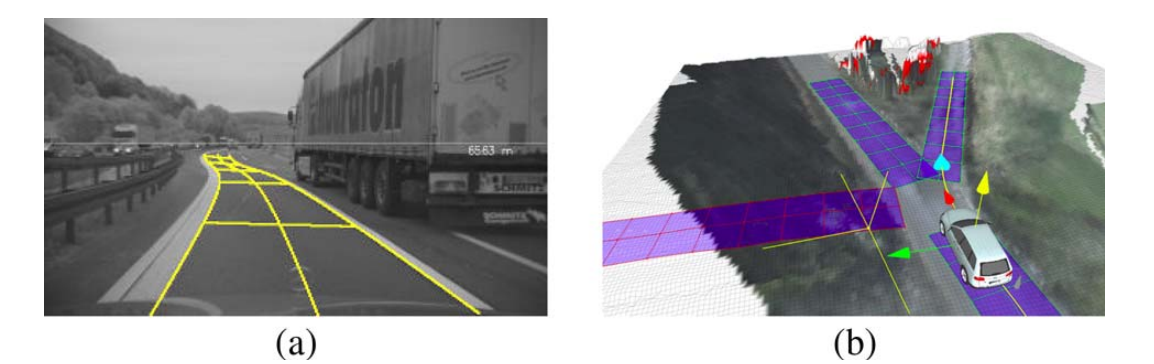
\includegraphics[width=0.8\linewidth]{img/5-1}
	\caption{5G NR 帧结构示例}
	\label{fig:5-1}
\end{figure}

下面我们概述感知网络的基本框架及其所涉及的技术问题。为便于理解，我们的讨论基于通用蜂窝网络，即感知移动网络（PMN）。

\subsection{利用 5G 及未来波形进行感知的可行性}

在本小节中，我们将深入探讨使用 5G 及未来波形进行感知的可行性，以及其中的挑战和机遇。

在ISAC系统的任何感知操作模式下，已知的参考信号都是必不可少的。它既可以用于对接收到的回波信号进行匹配滤波，从而提取目标信息，也可以用于减轻随机通信数据的影响。在 4G LTE 和 5G NR 中，OFDM ( 正交频分复用 )是默认的波形格式，可以通过遵循第四节 B 部分概述的通用信号处理流程，在 PMN 中利用 OFDM 进行感知，通过逐元素除法消除了回波信号中的数据依赖性。这要求接收端在感知目标之前已知发射端发送的通信信号，因此需要考察通信帧内可用于感知的信号资源。

让我们研究 NR 的标准帧结构，该结构基于 3GPP 技术规范 38.211 Release 15 \cite{8928165}，如图 2 所示。一个 5G NR 帧时长为 $10~\text{ms}$，由 10 个子帧组成，每个子帧的持续时间为 $1~\text{ms}$。每个子帧包含 $2^\mu$ 个时隙，其中 $\mu$ 是从 0 到 5 的参数集（numerology），对应于 $2^\mu \cdot 15~\text{kHz}$ 的子载波间隔。每个时隙占用 14 或 12 个 OFDM 符号，这取决于使用的是常规 CP 还是扩展 CP。

SSB（同步信号块）中包含的信号对于基站 (BS) 和用户设备 (UE) 都是已知的，可以很容易地被利用进行感知。特别是，同步信号（即 PSS 和 SSS）通常具有固定结构，而 PBCH（物理广播信道）及其 DMRS 则更加灵活，可以通过专门定制的预编码和调度方案针对通信与感知 (S\&C) 进行联合优化。此外，NR Release 16 中定义的定位参考信号 (PRS) 也可以随时用于定位。这些设计仅利用帧结构的一部分进行感知，按照全统一波形的设计理念，可以进一步利用帧中可用的数据负载进行感知，这将显著提高匹配滤波增益和感知信噪比 (SNR)。

\subsection{利用 5G 及未来波形进行感知的挑战与机遇}

根据上述分析，我们接下来将讨论 5G NR 波形级 ISAC 设计中遇到的关键挑战及其潜在解决方案。

\textit{a) 高精度感知的带宽受限：} 3GPP 为 NR 定义了两种频率范围 (FR) 类型。FR1 (Sub-6 GHz) 范围从 $450~\text{MHz}$ 到 $6~\text{GHz}$，FR2 (mmWave) 范围从 $24.25~\text{GHz}$ 到 $52.6~\text{GHz}$。根据式 (20)，FR1 的信道带宽最高为 $100~\text{MHz}$，FR2 最高为 $400~\text{MHz}$，分别对应 $1.5~\text{m}$ 和 $0.375~\text{m}$ 的距离分辨率。虽然这些分辨率对于基础感知服务可能已经足够，但它们无法满足自动驾驶等需要 $0.1~\text{m}$ 级感知分辨率的高精度应用需求。

提高距离分辨率的一种可能途径是利用载波聚合 (CA) 技术，该技术能够通过为同一用户分配多个频块来提高数据速率。本着这种精神，也可以分配多个频块来感知同一目标。例如，如果在 Sub-6 GHz 频段内聚合 16 个载波，总带宽可达 $1.6~\text{GHz}$，从而实现 $0.094~\text{m}$ 的距离分辨率。然而，如果聚合的带宽是不连续的，可能会出现较高的距离旁瓣 (range sidelobes)\cite{7096298}，从而导致较高的虚警概率。为此，应采取适当措施降低旁瓣。

\textit{b) 单站感知中的自干扰：} 对于单站 (mono-static) 感知操作，虽然 SSB 和数据负载都是已知的并可用于目标探测，但自干扰 (SI) 是一个无法回避的问题。让我们以 $\mu=4$ 的帧为例，此时子载波间隔为 $240~\text{kHz}$，相应的 OFDM 符号加 CP 持续时间为 $4.46~\mu\text{s}$。该持续时间对应于 $670~\text{m}$ 距离处的目标。也就是说，如果目标在 $670~\text{m}$ 范围内，当基站仍在发送信号时，其回波信号就已经反射回基站了。从发射机泄漏到接收机的信号会导致强烈的自干扰，使接收机的放大器饱和并掩盖目标回波。对于运动目标，只要基站能在多普勒频谱上将其区分开，自干扰的危害可能较小。然而，对于静态目标，即使只使用单个 OFDM 符号，这也会导致 $100$--$1000~\text{m}$ 级别的“盲区” (black zone)。

\textit{c) 双基地感知中的未知数据负载：} 对于发射机和接收机分离的双基地 (bi-static) 感知，自干扰不再是问题，已知的 SSB 信号可以直接用作感知波形。然而，由于接收端可能不知道数据负载（尤其是在发射机和接收机之间没有直接信道/链路的情况下），因此无法直接利用数据负载。为了解决这个问题，接收机可以首先利用 SSB 信号中已知的 PBCH（物理广播信道）估计信道矩阵，然后使用估计的信道解调数据符号。这样，解调后的符号就可以与 SSB 信号结合使用，用于估计目标参数。